\chapter{Related Work}
\label{Related Works}

Citation analysis is broad field of study, which has recently attracted computational methodology, using natural language and machine learning techniques for automation.  We categorise such recent past works into several directions for development.  A subfield of study that has a major impact is citation classification (similarly named as citation function). Such work aims to determine the basis for the authors' citation of the others' work, and thus better aid readers understand the key ideas presented in the paper. The reasons why authors would cite, are what was meant by the citation function. \outcite{teufel2006bannotation} defined an annotation scheme (see Figure~\ref{fig:teufelannotationscheme}) for citation function that is able to describe the relationships between documents linked via citations.

\begin{figure}[h]
\framebox[\textwidth]{
	\begin{tabular}{ l p{11cm}}
		\textsc{Category} & \textsc{Description}\\
		\hline
		Weak & Weakness of cited approach \\
		CoCoGM & Contrast/Comparison in Goals or Methods (neutral) \\
		CoCo- & Contrast/Comparison in Results (neutral)\\
		CoCoXY & Unfavourable Contrast/Comparison (current work is better than cited work)\\
		\hline
		PBas & author uses cited work as starting point \\
		PUse & author uses tools/algorithms/data \\
		PModi & author adapts or modifies tools/algorithms/data \\
		PMot & this citation is positive about approach or problem addressed (used to motivate work in current paper) \\
		PSim & author's work and cited work are similar \\
		PSup & author's work and cited work are compatible/provide support for each other \\
		\hline
		Neut & Neutral description of cited work, or not enough textual evidence for above categories or unlisted citation function
	\end{tabular}
}
\caption{12-class annotation scheme designed by \protect\outcite{teufel2006bannotation}}
\label{fig:teufelannotationscheme}
\end{figure}

\outcite{nakov2004citances} discussed the potential of using text surrounding citations, \textit{citances}, for automated analysis of bioscience literature.
%\outcite{teufel2006automatic} previously worked on the automatic classification of citation function, utilising features extracted from the
%\textit{citing context}. 
% Min: we need more detail about this work.  Features?  Classifiers?  Interesting observations?
\outcite{dongensemble} presented an approach to citation classification in which, they extracted several features from \textit{citances}. Some features worth mentioning are their \textit{physical features}, that included the number of unique references cited within the \textit{citances}, and one that measured the existence of cue words. \outcite{teufel2006automatic} also described a similar feature that involved cue phrases, a strong indicator for citation function. Together, these previous works demonstrated the importance of utilising \textit{citances} in citation analysis tasks.

%Similarly, authors worked on analysing the 
%% Min: define sentiment and polarity.  Won't be understandable to those not in NLP.
%sentiment of citations to determine the polarity of these citations. Most recently, \outcite{athar2011sentiment} used sentence structure based features extracted from the citing context to produce 
%% Min: give exact numbers and details on the datasets.
%promising results.

In \cite{citation-sensitive} and \cite{csibs}, Wan and his team built a research tool that acts as a reading aid for readers when browsing through scientific papers. \outcite{csibs} investigated the \textit{literature browsing task} through surveys on researchers who read scientific papers frequently to keep up-to-date themselves. In the initial study conducted by Wan {\it et al.}, several key ideas were revealed. First, when researchers read scientific papers and see citations made by the author, their main concern -- as time-constrained professionals -- is whether the cited paper is worth their effort to follow up on. At the same time, the researchers need to know whether to believe the claim made in the citation. Second, readers faced the difficulty of finding the exact text that justify the citation. Third, the surveys revealed that readers thought that it would be  useful if a reading tool could identify important sentences and key words in the cited paper. This study conducted by \outcite{csibs} is based on the fundamental idea of improving the reading experience of researchers. The goal was to save a reader's time by assisting in the relevance judgement process on the cited documents. As it is often that readers do need to read cited documents to gain insight on the current paper's context, this task is of relevance and importance. The authors then developed the {\it Context Sensitive In-Browser Summariser} (CSIBS) tool based on their studies. Figure~\ref{fig:wanscreenshot} is an overlay of the CSIBS that displays citation-sensitive previews of the cited document. While it highlights matching keywords related to the citation, these sentences on the overlay do not necessarily justify the citation. To locate the provenance solely by word overlap would prove to be ineffective as paraphrasing and re-organising of sentence structure are common when authors cite previous works. There is a need to consider aligning \textit{citances} to the cited document.

\begin{figure}[h]
  \centering
  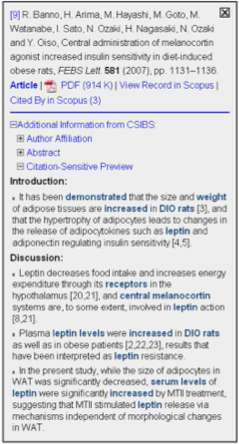
\includegraphics[scale=0.50]{./wanscreenshot}
  \caption{In-browser overlay preview of the CSIBS}
  \label{fig:wanscreenshot}
\end{figure}

% Min: you need a transition.  I didn't anticipate the topic change.  Why are you talking about paraphrasing and alignment (they are relevant, but why)?
Aligning sentences belonging to similar documents is an important research area for tasks related to summarisation and paraphrasing. \outcite{nelken2006towards} presented a novel algorithm for sentence alignment in for texts in a single language (i.e., monolingual corpora). They showed their approach, which is based on
% Min: need to briefly explain TF.IDF
TF$\times$IDF (a weighting scheme that reflects the importance of a word to a document in a collection of documents) similarity score, produced a high precision (83.1\%) for the task of aligning sentence.
%More recent work by \outcite{li2010fast} introduced a new sentence alignment algorithm called Fast-Champollion. Briefly, it splits the input text into alignment fragments and identifies the components of these fragments before aligning them using a
%% Min: this isn't clear.  Spell out or introduce the method at the high-level in 1-2 sentences.  Why is this related to your work?
%Champollion-based algorithm.
Adding to what we mentioned early, authors paraphrase the content they were referring to usually for greater clarity and to introduce variety. While \outcite{shinyama2002automatic} presented an approach to acquire paraphrase automatically, in our citation provenance project, we aim for the converse goal. By comparing the words and phrases used in a citation with paraphrases extracted from a cited work, one may achieve improved sentence alignment between the two documents.